\chapter{Design and Rationale - example middle chapter}

\section{Design}
Describe the design of the system at a high-level. The system should support the use cases described in the previous chapter.
\begin{figure}
    \centering
    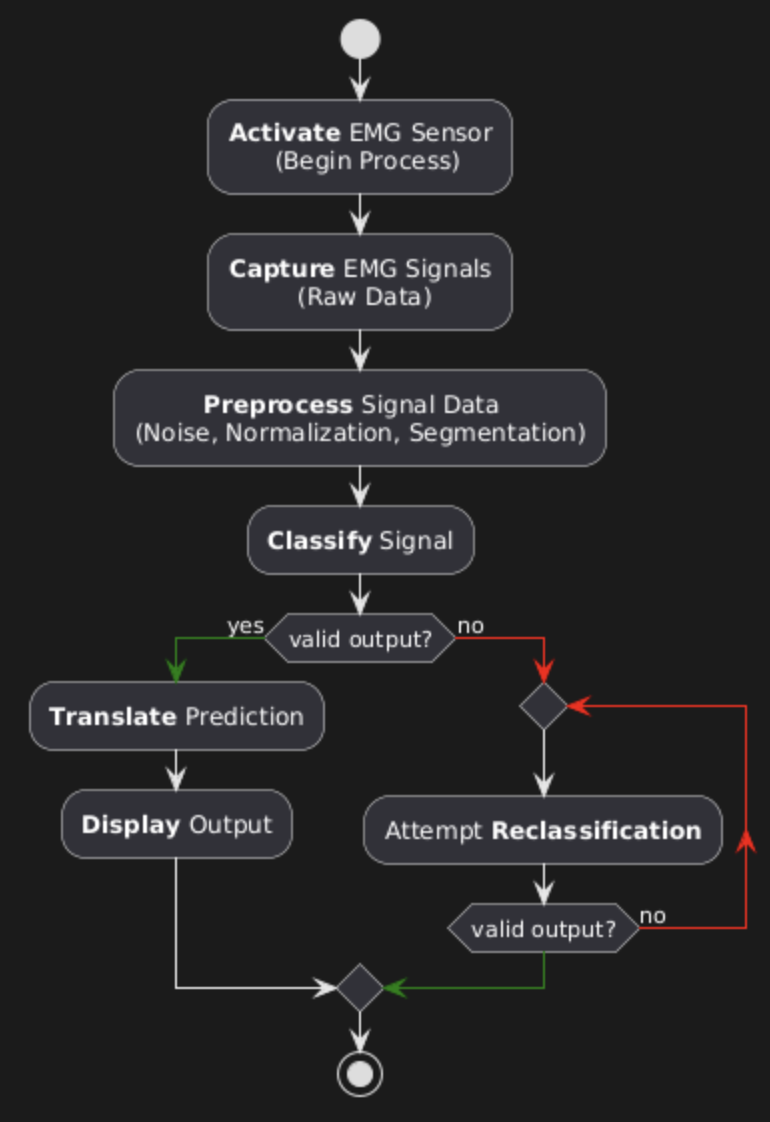
\includegraphics[width=0.5\linewidth]{Images/Activity_Diagram.png}
    \caption{Activity Diagram}
    \label{fig:enter-label}
\end{figure}
\begin{figure}
    \centering
    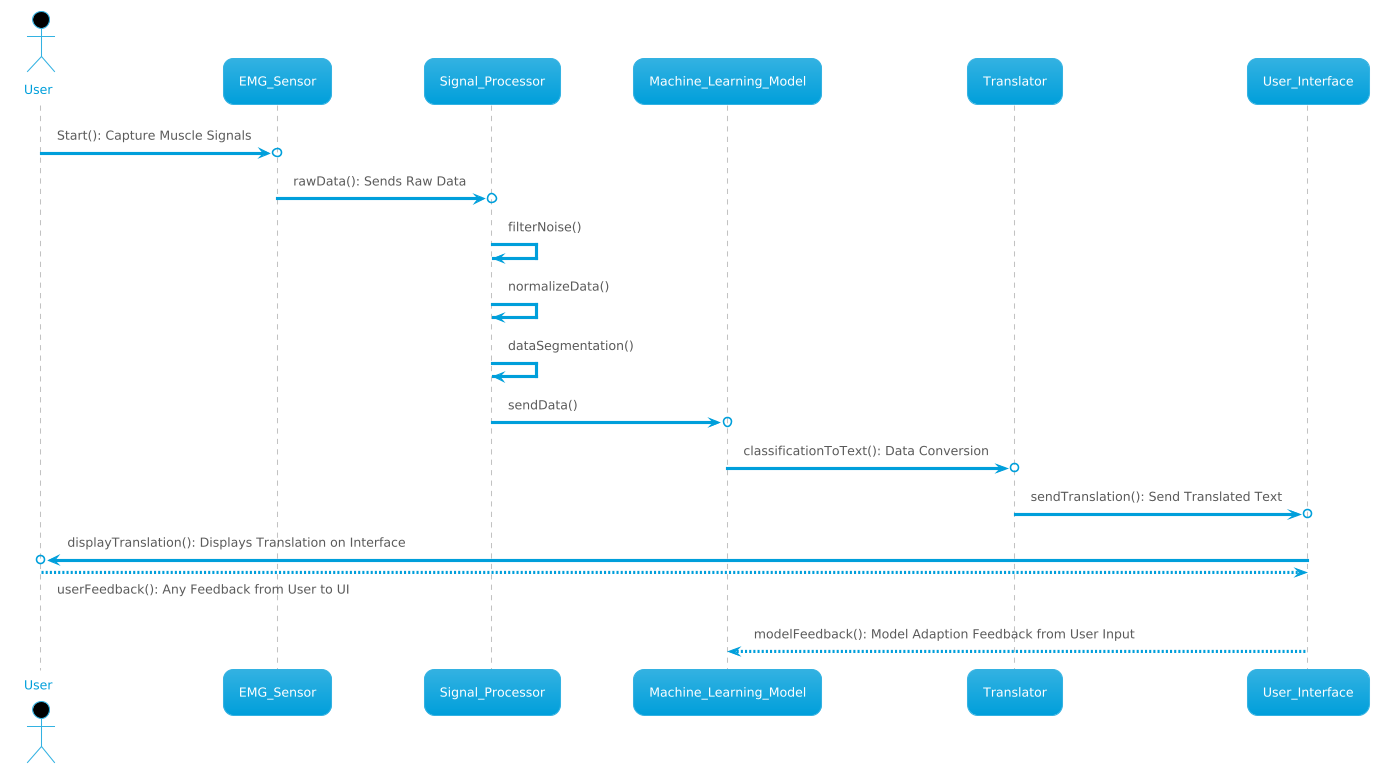
\includegraphics[width=0.75\linewidth]{Images/Sequence_Diagram.png}
    \caption{Sequence Diagram}
    \label{fig:enter-label}
\end{figure}
\begin{figure}
    \centering
    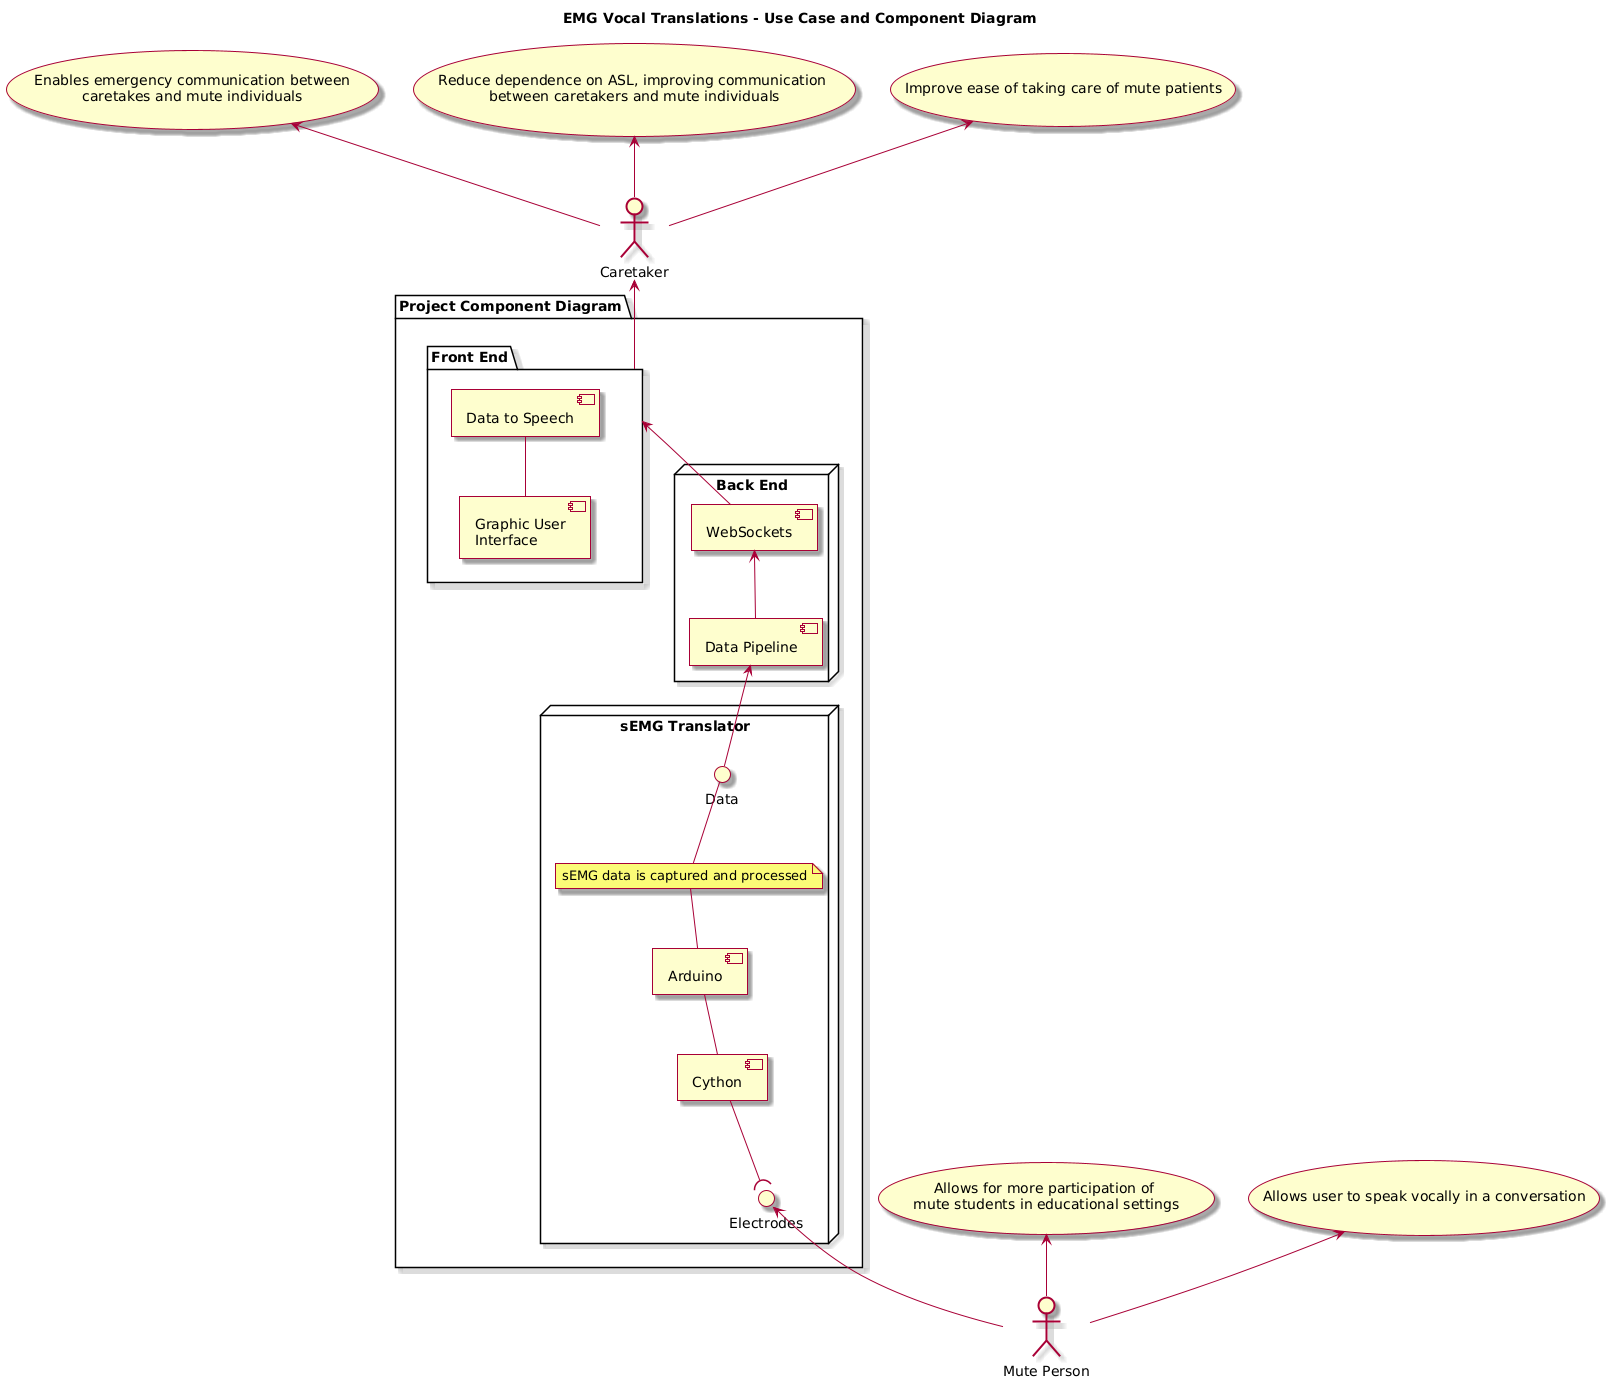
\includegraphics[width=1\linewidth]{Images/UML-2.png}
    \caption{Use Case Diagram}
    \label{fig:enter-label}
\end{figure}
\begin{figure}
    \centering
    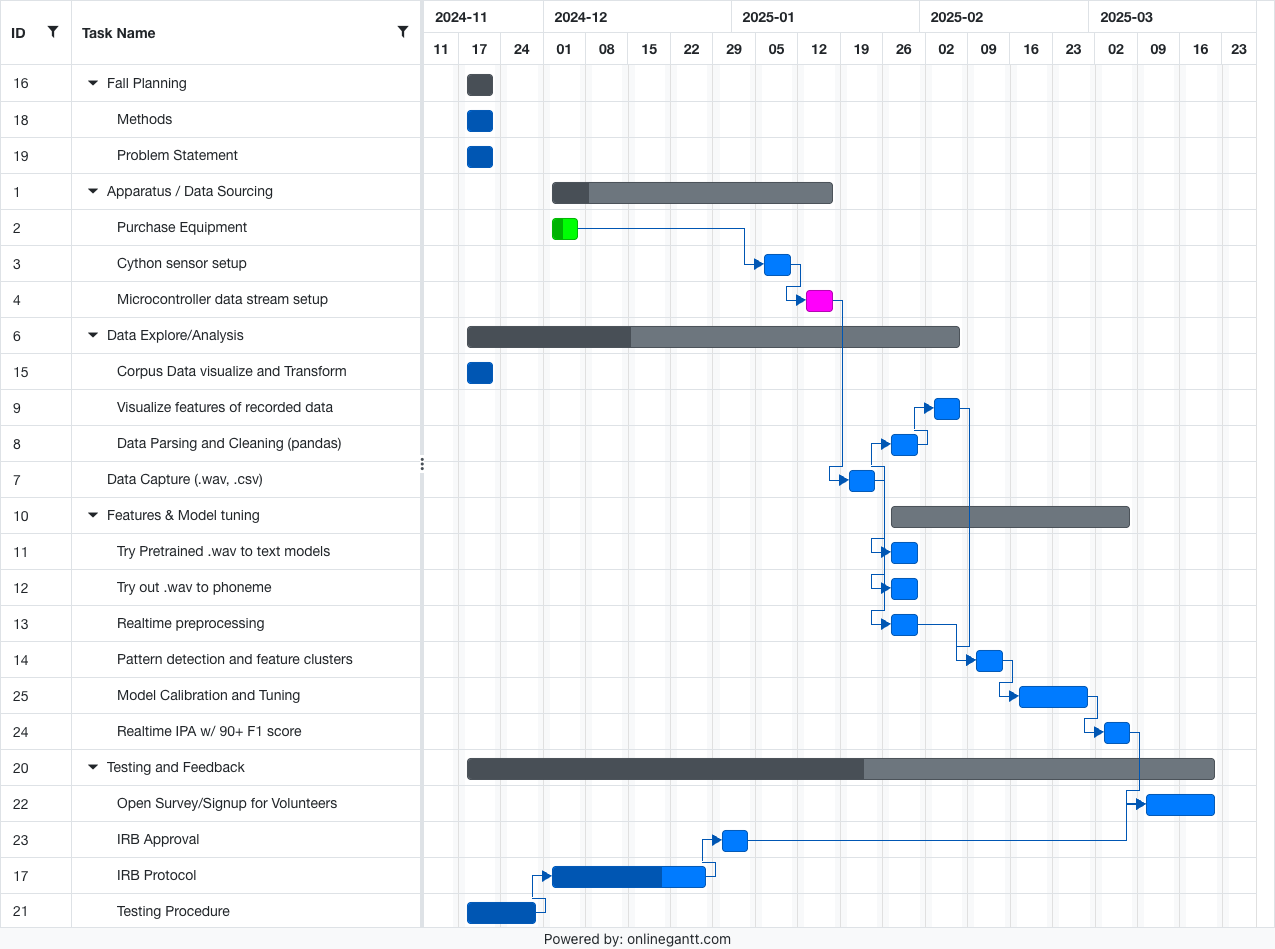
\includegraphics[width=1\linewidth]{Images/emg_vocal_gantt.png}
    \caption{Gantt Timeline}
    \label{fig:enter-label}
\end{figure}
---C4 system context and container diagrams go in this section. See: https://c4model.com/ (C4 Model Website)  ---

\section{Functional requirements}
Generally expressed in the form: "system must do $<$requirement$>$." These are similar to use cases (i.e, "the user can do XYZ"), but written from the perspective of the system. For example: "The landing page must introduce several different virtual tours and let the user choose one." \\
See https://en.wikipedia.org/wiki/Functional\textunderscore requirement

\section{Non-functional requirements}
Generally expressed in the form: "system shall be $<$requirement$>$." These are also known as quality requirements. For example: 
"The virtual tour shall be fast-to-load. That is, the tour itself and any embedded media in it should load quickly enough that it is not a major annoyance for our target users." \\
See https://en.wikipedia.org/wiki/Non-functional\textunderscore requirement

\section{Rationale}
Describe why the system is designed this way. What alternatives did you consider, and why is design a good choice.
